% Options for packages loaded elsewhere
\PassOptionsToPackage{unicode}{hyperref}
\PassOptionsToPackage{hyphens}{url}
%
\documentclass[
]{article}
\usepackage{amsmath,amssymb}
\usepackage{lmodern}
\usepackage{iftex}
\ifPDFTeX
  \usepackage[T1]{fontenc}
  \usepackage[utf8]{inputenc}
  \usepackage{textcomp} % provide euro and other symbols
\else % if luatex or xetex
  \usepackage{unicode-math}
  \defaultfontfeatures{Scale=MatchLowercase}
  \defaultfontfeatures[\rmfamily]{Ligatures=TeX,Scale=1}
\fi
% Use upquote if available, for straight quotes in verbatim environments
\IfFileExists{upquote.sty}{\usepackage{upquote}}{}
\IfFileExists{microtype.sty}{% use microtype if available
  \usepackage[]{microtype}
  \UseMicrotypeSet[protrusion]{basicmath} % disable protrusion for tt fonts
}{}
\makeatletter
\@ifundefined{KOMAClassName}{% if non-KOMA class
  \IfFileExists{parskip.sty}{%
    \usepackage{parskip}
  }{% else
    \setlength{\parindent}{0pt}
    \setlength{\parskip}{6pt plus 2pt minus 1pt}}
}{% if KOMA class
  \KOMAoptions{parskip=half}}
\makeatother
\usepackage{xcolor}
\IfFileExists{xurl.sty}{\usepackage{xurl}}{} % add URL line breaks if available
\IfFileExists{bookmark.sty}{\usepackage{bookmark}}{\usepackage{hyperref}}
\hypersetup{
  pdftitle={Pivot Tables},
  pdfauthor={Pairote Satiracoo},
  hidelinks,
  pdfcreator={LaTeX via pandoc}}
\urlstyle{same} % disable monospaced font for URLs
\usepackage[margin=1in]{geometry}
\usepackage{longtable,booktabs,array}
\usepackage{calc} % for calculating minipage widths
% Correct order of tables after \paragraph or \subparagraph
\usepackage{etoolbox}
\makeatletter
\patchcmd\longtable{\par}{\if@noskipsec\mbox{}\fi\par}{}{}
\makeatother
% Allow footnotes in longtable head/foot
\IfFileExists{footnotehyper.sty}{\usepackage{footnotehyper}}{\usepackage{footnote}}
\makesavenoteenv{longtable}
\usepackage{graphicx}
\makeatletter
\def\maxwidth{\ifdim\Gin@nat@width>\linewidth\linewidth\else\Gin@nat@width\fi}
\def\maxheight{\ifdim\Gin@nat@height>\textheight\textheight\else\Gin@nat@height\fi}
\makeatother
% Scale images if necessary, so that they will not overflow the page
% margins by default, and it is still possible to overwrite the defaults
% using explicit options in \includegraphics[width, height, ...]{}
\setkeys{Gin}{width=\maxwidth,height=\maxheight,keepaspectratio}
% Set default figure placement to htbp
\makeatletter
\def\fps@figure{htbp}
\makeatother
\setlength{\emergencystretch}{3em} % prevent overfull lines
\providecommand{\tightlist}{%
  \setlength{\itemsep}{0pt}\setlength{\parskip}{0pt}}
\setcounter{secnumdepth}{5}
\usepackage{booktabs}
\usepackage{amsthm}
\usepackage{LectureNoteMacro}
\usepackage{bbm}
\usepackage{mathtools}
\usepackage{tikz}
\makeatletter
\def\thm@space@setup{%
  \thm@preskip=8pt plus 2pt minus 4pt
  \thm@postskip=\thm@preskip
}
\makeatother
\ifLuaTeX
  \usepackage{selnolig}  % disable illegal ligatures
\fi
\usepackage[]{natbib}
\bibliographystyle{plainnat}

\title{\textbf{Pivot Tables}}
\author{Pairote Satiracoo}
\date{2021-09-24}

\usepackage{amsthm}
\newtheorem{theorem}{Theorem}[section]
\newtheorem{lemma}{Lemma}[section]
\newtheorem{corollary}{Corollary}[section]
\newtheorem{proposition}{Proposition}[section]
\newtheorem{conjecture}{Conjecture}[section]
\theoremstyle{definition}
\newtheorem{definition}{Definition}[section]
\theoremstyle{definition}
\newtheorem{example}{Example}[section]
\theoremstyle{definition}
\newtheorem{exercise}{Exercise}[section]
\theoremstyle{definition}
\newtheorem{hypothesis}{Hypothesis}[section]
\theoremstyle{remark}
\newtheorem*{remark}{Remark}
\newtheorem*{solution}{Solution}
\begin{document}
\maketitle

{
\setcounter{tocdepth}{2}
\tableofcontents
}
\hypertarget{dates-and-date-functions}{%
\section{Dates and date functions}\label{dates-and-date-functions}}

Dates and date functions will be discussed in this section. Depending on
the system setting, the dates used in this section corresponds to the
U.S. setting, i.e.~month/day/year. Thus, 7/1/2017 corresponds to 1 July
2017.

The following date formats are recognized by Excel:

\begin{itemize}
\item
  7/1/2017, 7/1/17
\item
  7-1-2017, 7-1-17,
\item
  7-1/2017, 7-1/17,
\item
  July 1, 2017
\item
  1-Jul-2017
\end{itemize}

if the date input is without the year, then it is the date on the
current year, i.e.~7-1, 7/1, July 1, Jul 1, corresponds to 1 July 2018.

\hypertarget{inconsistent-date-entries}{%
\subsection{Inconsistent date entries}\label{inconsistent-date-entries}}

\begin{example}
\protect\hypertarget{exm:unlabeled-div-1}{}\label{exm:unlabeled-div-1}

\emph{What will be the output when we enter dates by using the
following two digits for the years:}

\begin{enumerate}
\def\labelenumi{\arabic{enumi}.}
\item
  \emph{7/1/01}
\item
  \emph{7/1/60}
\end{enumerate}

\end{example}

Excel interprets two digit years between 00 and 29 as 21st century
dates, and two digit years between 30 and 99 as 20th century dates.

\hypertarget{date-serial-number}{%
\subsection{Date serial number}\label{date-serial-number}}

Excel stores dates as sequential serial numbers so that they can be used
in calculations. For example,

\begin{itemize}
\item
  1 January 1900 is serial number 1,
\item
  1 January 2018 is serial number 43101 because it is 43101 days after
  1 January 1900.
\end{itemize}

\hypertarget{date-functions}{%
\subsection{Date functions}\label{date-functions}}

The list of date functions can be seen by choosing

\textbf{Formulas \(\rightarrow\) Function Library \(\rightarrow\) Function Library \(\rightarrow\) Date \& Time}.

\begin{longtable}[]{@{}ll@{}}
\toprule
\textbf{Function} & \textbf{Description} \\
\midrule
\endhead
DATE & Returns the serial number of a particular date \\
DATEVALUE & Converts a date in the form of text to a serial number \\
DAY & Converts a serial number to a day of the month \\
DAYS & Returns the number of days between two dates \\
WEEKDAY & Converts a serial number to a day of the week \\
NETWORKDAYS & Returns the difference between two dates, excluding weekend days (Saturdays and Sundays) \\
WORKDAY & Returns a number that represents a date that is the indicated number of working days before or after a date (the starting date) \\
EDATE & Returns the serial number that represents the date that is the indicated number of months before or after a specified date \\
EOMONTH & Returns the serial number for the last day of the month that is the indicated number of months before or after a specified date \\
YEARFRAC & Returns a decimal value that represents fractional years between two dates \\
\bottomrule
\end{longtable}

For a complete list, see the date and time functions available online.
More detailed examples are also given in the Excel lab.

\hypertarget{working-with-texts}{%
\section{Working with Texts}\label{working-with-texts}}

In this section, we will see how Excel handles text strings, and how we
use text functions to modify and manipulate text strings. First, we give
a note regarding texts in Excel.

\begin{itemize}
\item
  A single cell can hold up to 32,000 characters. In case you need to
  display a lot of text in a worksheet, then use a text box (Choose
  Insert \(\Rightarrow\) Text \(\Rightarrow\) Text Box). It will be easier
  to edit texts in the text box than in cells.
\item
  Sometimes, when you download numerical data from the internet or
  database, the imported values are treated as text, i.e.~when you do
  a calculation with such data, you will get a \#VALUE error. When a
  number is not treated as a number, there will be an error indicator.
  By clinking to expand a list of options, you can then convert it to
  the number.
\item
  Another issue that you may encounter is about currency that uses
  different characters to separate thousands or decimals.
  \url{https://en.wikipedia.org/wiki/Decimal_separator}
\end{itemize}

\hypertarget{text-functions}{%
\subsection{Text functions}\label{text-functions}}

The following Excel functions can be used to modify text strings in the
format you need. Alternatively, one may extract data by using the
Convert Text To Columns Wizard (choose Data \(\Rightarrow\) Text To
Columns).

\begin{enumerate}
\def\labelenumi{\arabic{enumi}.}
\item
  RIGHT(text,{[}n{]}) returns the last \(n\) characters in a text string.
\item
  LEFT(text, {[}n{]}) returns the first \(n\) characters in a text string.
\item
  MID(text, start\_num, num\_chars) returns num\_char characters from a
  text string, starting at start\_num.
\item
  TRIM(text) removes all spaces from text except for single spaces
  between words. Use TRIM when text strings have irregular spacing.
\item
  LEN(text) returns the number of characters in a text string.
\item
  FIND(find\_text, within\_text, {[}start\_num{]}) return the location at
  or after character start\_num of the first character of find\_text in
  within\_text.
\item
  SEARCH(find\_text, within\_text, {[}start\_num{]}) has the same syntax as
  FIND, but it is not case sensitive.
\item
  SUBSTITUTE(text, old\_text, new\_text, {[}instance\_num{]}) is used to
  replace new\_text for old\_text in a text string. Here Instance\_num is
  optional. It specifies which occurrence of old\_text you want to
  replace with new\_text. If you specify instance\_num, only that
  instance of old\_text is replaced. Otherwise, every occurrence of
  old\_text in text is changed to new\_text.
\end{enumerate}

\hypertarget{character-codes}{%
\subsection{Character codes}\label{character-codes}}

Excel uses the standard ASCII character set. Therefore, each character
has its own code. For example, to get the code number of ``A'', simply
type

=CODE(``A''), which returns the code number 65.

The CHAR function reverses the role of CODE function, i.e.

=CHAR(65), which returns the letter A. The input for the CHAR function
should be a value between 1 and 255.

For the complete list of ASCII codes, please visit
\url{https://theasciicode.com.ar}

\begin{example}
\protect\hypertarget{exm:unlabeled-div-2}{}\label{exm:unlabeled-div-2}

\emph{Create an Excel file to list all the first 255 ASCII
codes. It is a good idea to compare the outputs with those from the
website above.}

\end{example}

\hypertarget{determining-whether-two-string-are-identical}{%
\subsection{Determining whether two string are identical}\label{determining-whether-two-string-are-identical}}

In order to determine whether strings in cell A1 and A2 have the same
contents, we use = A1 = A2, which returns either TRUE or FALSE. Note
that the comparison is not case-sensitive.

Alternative, the function that provides an exact, case-sensitive
comparison is EXACT function.

\hypertarget{joining-two-or-more-cells}{%
\subsection{Joining two or more cells}\label{joining-two-or-more-cells}}

To join two or more cells, Excel uses an ampersand \&. For example if the
string ``the effective interest rate per annum'' is in A1 and the value of
5\% (formatted value) is in B1. Then use the formula

= A1 \& '' is '' \& B1, which returns the effective interest rate per annum
is 0.05.

A better solution is to use the TEXT function to format the value as
text as follows.

= A1 \& '' is '' \& TEXT(B1,'' 0.00\%``) , which returns the effective interest
rate per annum is 0.05.

Use \textbf{Home Format Format cells} to obtain the list of various text
formats.

For example, if A1 contains the principle of \$10,000, then

= ``The principle is'' \& TEXT(A1, '' \$\#,\#\#0''), which returns The
principle is \$10,000.

The following table gives examples that are format with TEXT function.

\begin{verbatim}
=TEXT(1234.567,"$#,##0.00")     
Currency with a thousands separator and 2 decimals, like $1,234.57. Note that Excel rounds the value to 2 decimal places.

=TEXT(TODAY(),"MM/DD/YY")
Today's date in MM/DD/YY format, like 03/14/12

=TEXT(TODAY(),"DDDD")
Today's day of the week, like Monday

=TEXT(NOW(),"H:MM AM/PM")
Current time, like 1:29 PM

=TEXT(0.285,"0.0%")
Percentage, like 28.5%

=TEXT(4.34 ,"# ?/?")
Fraction, like 4 1/3

=TRIM(TEXT(0.34,"# ?/?"))
Fraction, like 1/3. Note this uses the TRIM function to remove the leading space with a decimal value.

=TEXT(12200000,"0.00E+00")
Scientific notation, like 1.22E+07

=TEXT(1234567898,"[<=9999999]###-####;(###) ###-####")
Special (Phone number), like (123) 456-7898

=TEXT(1234,"0000000")
Add leading zeros (0), like 0001234
\end{verbatim}

The TEXT function will convert numbers to text. It is best practice to
keep your original values in one cell, and formatted number in another
cell. When you do calculation, you should refer to the cells containing
original values.

\hypertarget{interest-rate-present-values-and-cashflows}{%
\section{Interest Rate, Present Values and Cashflows}\label{interest-rate-present-values-and-cashflows}}

\hypertarget{working-with-a-single-cashflow-in-excel}{%
\subsection{Working with a single cashflow in Excel}\label{working-with-a-single-cashflow-in-excel}}

\hypertarget{how-to-calculate-the-future-value-of-a-single-cashflow}{%
\subsubsection{How to calculate the future value of a single cashflow}\label{how-to-calculate-the-future-value-of-a-single-cashflow}}

Suppose an amount \(C\) is deposited in an account that pays a fixed
interest at the rate of \(i\)\% per time units. Then after \(t\) time units,
the deposit will have accumulated to \[C (1+i)^t.\]

In Excel, the function FV calculates the future value of a single
investment (and also periodic constant payments) and a constant interest
rate.

The syntax of the function is:

\[\text{FV(rate, nper, pmt, [pv], [type])},\]

where

\begin{itemize}
\item
  rate is the interest rate per period
\item
  nper is the number of periods over which the investment is made.
\item
  pmt (used for an annuity type) is the payment made each period and
  cannot change over the life of the annuity.
\item
  pv (optional) is an additional cash flow now (time 0)
\item
  fv is an additional cash flow nper periods from now.
\item
  type (optional) is an optional argument that defines whether the
  payment is made at the start or the end of the period:

  0 - the payment is made at the end of the period;

  1 - the payment is made at the start of the period.

  If the {[}type{]} argument is omitted, it takes on the default value
  of 0.
\end{itemize}

The following timeline illustrates the cashflows used for the FV
function (assuming that the payments (pmt) are made in arrears).

\begin{figure}

{\centering 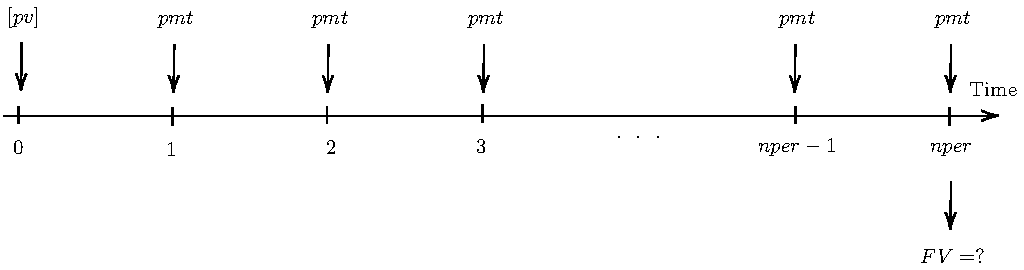
\includegraphics{SCMA329ExcelBookdownproj_files/figure-latex/tikz-ex-1} 

}

\caption{Timeline of cashflows for FV function}\label{fig:tikz-ex}
\end{figure}

\textbf{Note} For a single cash flow, we set pmt argument to be 0, as there are no
ongoing payments after the initial investment.

\begin{example}
\protect\hypertarget{exm:unlabeled-div-3}{}\label{exm:unlabeled-div-3}

\emph{You plan to invest today with an interest rate of 3\% per
year effective. How much money will you accumulate at the end of 2
years?}

\end{example}

\textbf{Solution:} The accumulation of today in 2 years can be calculated by Excel as
\[\text{FV}(3\%, 2, 0, -100).\]

\hypertarget{how-to-calculate-the-present-value-of-a-single-cashflow}{%
\subsubsection{How to calculate the present value of a single cashflow}\label{how-to-calculate-the-present-value-of-a-single-cashflow}}

Similarly, the present value of a future cashflow \(C\) required at time
\(t\) time units at a fixed interest of \(i\)\% per time units can be
calculated as \[\frac{C}{(1+i)^t}.\] In Excel, the function PV
calculates the present value of a single investment (and also periodic
constant payments) and a constant interest rate. The syntax of the
function is:

\[\text{PV(rate, nper, pmt, [fv], [type])}\] where fv is an additional
cash flow nper periods from now.

\begin{example}
\protect\hypertarget{exm:unlabeled-div-4}{}\label{exm:unlabeled-div-4}

\emph{How much should you deposit into the account with an
interest of 8\% so that 10 years from now its value would be ?}

\end{example}

\textbf{Solution:}
The present value of today in 10 years can be calculated by Excel as
\[\text{PV}(8\%, 10, 0, -1000).\]

\hypertarget{present-values-of-a-series-of-cashflows}{%
\subsection{Present values of a series of cashflows}\label{present-values-of-a-series-of-cashflows}}

Consider a series of cashflows defined by

\begin{enumerate}
\def\labelenumi{\arabic{enumi}.}
\item
  the times of payments (cashflows), denoted by \(t_1, t_2, \ldots,\)
  and
\item
  the amount of payments, denoted by \(C_{r}\) (in short for \(C_{t_r}\)),
  which will be paid at time \(t_r\), for \(r = 1,2, \ldots\). The amounts
  can be positive or negative
\end{enumerate}

The present value at any time \(t\) of this series of cashflow is
\[PV(t) = \sum_{r=1}^\infty C_r (1 + i)^{t - t_r} = \sum_{r=1}^\infty C_r v^{t _r - t}\]
where \(i\) is the effective rate of interest and \(v = 1/(1+i)\).

\begin{figure}

{\centering 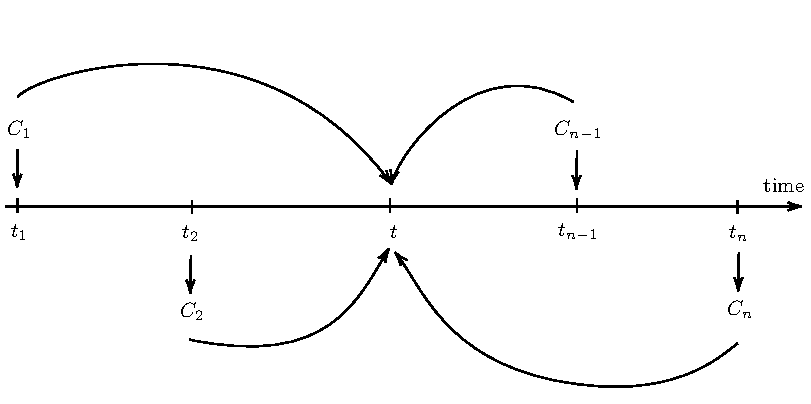
\includegraphics{SCMA329ExcelBookdownproj_files/figure-latex/tikz-ex2-1} 

}

\caption{Timeline of a series of cashflows}\label{fig:tikz-ex2}
\end{figure}

\textbf{Notes}
1. At a fixed effective rate of interest, the original series of
cashflows is equivalent to a single payment of amount \(PV(t)\) at
time \(t\).

\begin{enumerate}
\def\labelenumi{\arabic{enumi}.}
\setcounter{enumi}{1}
\tightlist
\item
  If two different series of cashflows have the same \(PV\) at one time
  at a given effective rate of interest, then they have the same \(PV\)
  at any time at that effective rate of interest.
\end{enumerate}

\hypertarget{level-annuities-certain}{%
\subsubsection{Level Annuities certain}\label{level-annuities-certain}}

An \emph{annuity} is a regular series of payments (cashflows). When the
payments are certain which are payable for a definite period of time, we
call it an \emph{annuity certain}.

\begin{itemize}
\item
  If the payments are made at the end of each time period, they are
  paid \emph{in arrear}.
\item
  Otherwise, payments are made at the beginning of each time period,
  they are pain \emph{in advance}.
\item
  An annuity paid in advance is also known as an \emph{annuity due}
\item
  If each payment is for the same amount, this is a \emph{level} annuity.
\end{itemize}

\begin{example}
\protect\hypertarget{exm:unlabeled-div-5}{}\label{exm:unlabeled-div-5}

\emph{Let \(i\) be the constant effective rate of interest per
time unit. In Excel, one can calculate the accumulated value of a level
annuity certain having cashflow of pmt unit at the end of each of the
next \(n\) time units by \[\text{FV}(i\%, n, pmt, 0).\] The cashflows of
this annuity is shown in the timeline below.}

\begin{figure}

{\centering 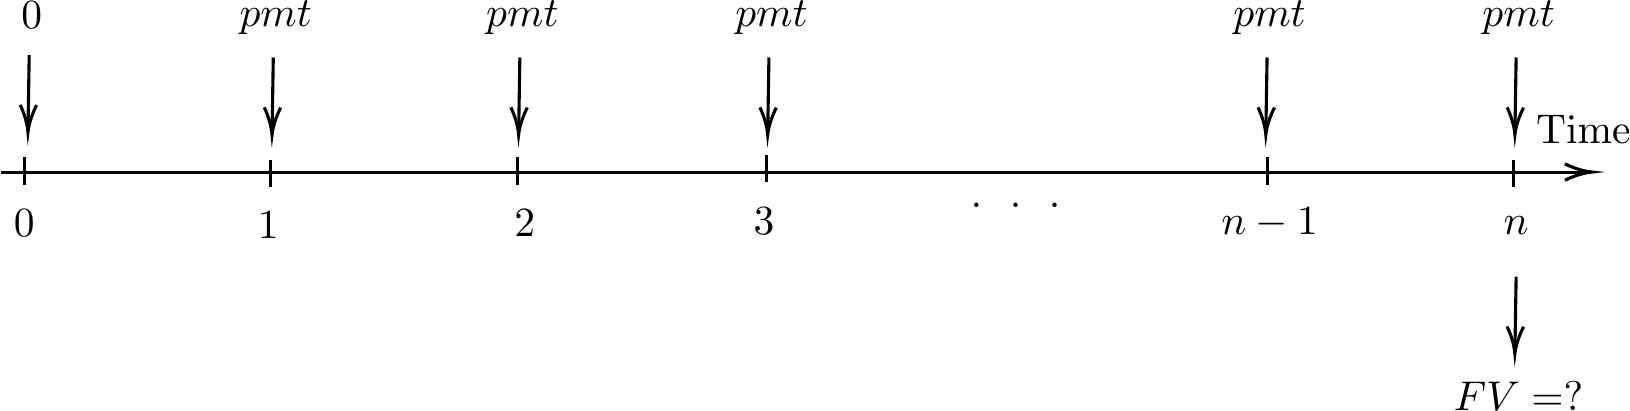
\includegraphics{SCMA329ExcelBookdownproj_files/figure-latex/tikz-ex3-1} 

}

\caption{Level Annuity Certain}\label{fig:tikz-ex3}
\end{figure}

\textbf{Note}
\emph{The last argument of the above syntax, {[}pv{]} (optional) which is an
additional cash flow now (at time 0), has been set to 0.}

\end{example}

\begin{example}
\protect\hypertarget{exm:unlabeled-div-6}{}\label{exm:unlabeled-div-6}

\emph{Let \(i\) be the constant effective rate of interest per
time unit. In Excel, one can calculate the present value at time 0 of a
level annuity certain having cashflow of pmt unit at the end of each of
the next \(n\) time units by \[\text{PV}(i\%, n, pmt, 0).\]}

\end{example}

The timeline of these cashflows is shown in the figure below:

\begin{figure}

{\centering 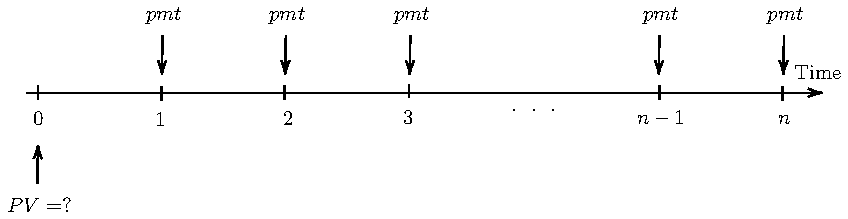
\includegraphics{SCMA329ExcelBookdownproj_files/figure-latex/tikz-ex4-1} 

}

\caption{Level Annuity Certain}\label{fig:tikz-ex4}
\end{figure}

\textbf{Note}
The last argument of the above syntax, {[}fv{]} (optional) which is an
additional cash flow at time \(n\), has been set to 0.

\begin{example}
\protect\hypertarget{exm:unlabeled-div-7}{}\label{exm:unlabeled-div-7}

\emph{Given the effective rate of interest of \(8\%\) p.a., use
Excel to calculate}

\begin{enumerate}
\def\labelenumi{\arabic{enumi}.}
\item
  \emph{the accumulation at 12 years of payable yearly in arrear for the
  next 12 years.}
\item
  \emph{the present value now of ,000 payable yearly in arrear for the next
  6 years.}
\item
  \emph{the present value now of ,000 payable half-yearly in arrear for the
  next 12.5 years.}
\end{enumerate}

\end{example}

\begin{example}
\protect\hypertarget{exm:unlabeled-div-8}{}\label{exm:unlabeled-div-8}

\emph{Let \(i = 4\%\) effective per time unit. Cashflows are
given as follows:}

\begin{itemize}
\item
  \emph{\(C_1 = 200\) at time \(t_1 = 1\).}
\item
  \emph{\(C_2 = 300\) at time \(t_2 = 3\).}
\item
  \emph{\(C_3 = -100\) at time \(t_3 = 5\).}
\item
  \emph{\(C_4 = -50\) at time \(t_4 = 6\).}
\end{itemize}

\emph{Develop the model using Excel to calculate}

\begin{enumerate}
\def\labelenumi{\arabic{enumi}.}
\item
  \emph{the accumulation at time \(t = 7\).}
\item
  \emph{the present value at time \(t = 0\).}
\item
  \emph{the present value at time \(t = 4\).}
\end{enumerate}

\end{example}

\hypertarget{lookup-formulas-and-data-tables}{%
\section{Lookup Formulas and Data Tables}\label{lookup-formulas-and-data-tables}}

\hypertarget{lookup-function}{%
\subsection{Lookup function}\label{lookup-function}}

Lookup function can be used to return (or retrieve) a value from a table
or a range of data. For example, use lookup function to find some
information such as date of birth, address etc. from a customer
database. Two useful lookup functions are \texttt{VLOOKUP} and \texttt{HLOOKUP}.

\begin{itemize}
\item
  The \texttt{VLOOKUP} function searches a value in the first column and
  returns a value in the same row from a column you specify in the
  table or array.
\item
  The \texttt{HLOOKUP} function searches a value in the top row and returns a
  value in the same column from a row you specify in the table or
  array.
\end{itemize}

The syntaxes for the \texttt{LOOKUP} functions are

\texttt{=VLOOKUP(lookup\ value,\ range\ containing\ the\ lookup\ value,\ the\ column\ number\ in\ the\ range\ containing\ the\ return\ value,\ {[}range\_lookup{]})}.

\texttt{=VLOOKUP(lookup\_value,\ table\_array,\ col\_index\_num,\ {[}range\_lookup{]})}.

\texttt{=HLOOKUP(lookup\_value,\ table\_array,\ row\_index\_num,\ {[}range\_lookup{]})}.

The \texttt{{[}range\_lookup{]}} is an optional which can be specified as \texttt{TRUE} for
approximate match or \texttt{FALSE} for an exact match.

\textbf{Notes}

\begin{enumerate}
\def\labelenumi{\arabic{enumi}.}
\item
  The EXCEL \texttt{LOOKUP} functions treat empty cells in the result range as
  \textbf{zeros}.
\item
  If the range\_lookup is \texttt{FALSE} and an exact match is not found, the
  function returns \#N/A.
\item
  If the range\_lookup is \texttt{TRUE} or omitted, the first column of the
  \texttt{VLOOKUP} table must be in ascending order. If lookup\_value is smaller
  than the the smallest value in the first column of the table\_array,
  then the function returns \#N/A.
\item
  Use \texttt{IFERROR} function to avoid the return \#N/A. Use the following
  syntax

  \texttt{=IFERROR(value,\ value\_if\_error)}

  (for example, \texttt{=IFERROR(VLOOKUP(...),"Value\ is\ not\ availble"} )
\item
  The wildcard character * and ? can be used when the range\_lookup
  argument is text.
\item
  The wildcard character ? refers to any single character, for example
  "analy?e" finds "analyse" and "analyze".
\item
  The wildcard character * refers to any number of characters, for
  example "bio*" finds "biology" and "biotechnology".
\end{enumerate}

\begin{example}
\protect\hypertarget{exm:unlabeled-div-9}{}\label{exm:unlabeled-div-9}

Import SET Index historical daily data starting from 1 January 2020 up
to now from
\url{https://www.investing.com/indices/thailand-set-historical-data}. Use
\texttt{LOOKUP} function to create the table showing

\begin{enumerate}
\def\labelenumi{\arabic{enumi}.}
\item
  the closing price on the first working day of each month (not
  including holidays).
\item
  the closing price on the last working day of each month (not
  including holidays).
\end{enumerate}

Hint: use

\texttt{=WORKDAY(DATE(YEAR(A1),MONTH(A1),1)-1,1)} to return the first working day
of a month and

\texttt{=WORKDAY(DATE(YEAR(A1),MONTH(A1)+1,1),-1)} to return the last working day
of a month.

\end{example}

\begin{example}
\protect\hypertarget{exm:unlabeled-div-10}{}\label{exm:unlabeled-div-10}

Use the SET Index historical data above. On your selected cells, find
the lowest and highest closing prices and the dates when those occurred
(sorting data is not allowed).

\end{example}

\hypertarget{match-and-index-functions}{%
\subsection{MATCH and INDEX functions}\label{match-and-index-functions}}

The \texttt{MATCH} and \texttt{INDEX} functions are often used together to perform
lookups.

The \texttt{MATCH} function returns the relative position of a specified item in
a range of cells. For example, if the range A1:A3 contains the values 2,
4 and 6, then the formula

\texttt{=MATCH(4,A1:A3,0)} returns the number 2, i.e.~the second item in the
range.

The syntax for MATCH is

\texttt{=MATCH(lookup\_value,\ lookup\_array,\ {[}match\_type{]})}

The optional argument is match\_type consisting of 3 values, \(-1\), 0 and
1, that specify how the match is determined.

\begin{itemize}
\item
  If match\_type = 1 or omitted, then \texttt{MATCH} finds the largest value
  less than or equal to lookup\_value where lookup\_array must be in
  \textbf{ascending order}.
\item
  If match\_type = 0, then \texttt{MATCH} finds the \textbf{first value exactly equal
  to} lookup\_value.
\item
  If match\_type = \(-1\), then MATCH finds the smallest value greater
  than or equal to lookup\_value where lookup\_array must be in
  \textbf{descending order}.
\end{itemize}

The \texttt{INDEX} function returns a value from within a table or range. The
syntax for INDEX is

\texttt{=INDEX(array,\ row\_num,\ {[}column\_num{]})}

If array contains only one row or column, the corresponding row\_num or
column\_num argument is optional.

\hypertarget{data-tables}{%
\subsection{Data tables}\label{data-tables}}

Data tables allows you to create a table of values from

\begin{itemize}
\item
  a formula as one or two variables from the formula are varied, and
\item
  more formulas for various values of a single input cell.
\end{itemize}

As a result, you can examine a range of possible values when one or two
variables are systematically changed. For example, a data table can be
used to display the amount your investment will grow to for various
numbers of compounding.

\begin{example}
\protect\hypertarget{exm:unlabeled-div-11}{}\label{exm:unlabeled-div-11}

An amount of \(P\) is invested for \(n\) years at a nominal interest rate of
i\%. Create a worksheet to calculate the effective annual interest rate
you will earn and the accumulation at time \(n\) years for various numbers
of compounding periods per year including

\begin{enumerate}
\def\labelenumi{\arabic{enumi}.}
\item
  annual compounding
\item
  semi-annual compounding
\item
  quarterly compounding
\item
  monthly compounding
\item
  bi-weekly compounding
\item
  weekly compounding
\item
  daily compounding
\end{enumerate}

\end{example}

\hypertarget{model-formulation}{%
\subsubsection*{Model formulation}\label{model-formulation}}
\addcontentsline{toc}{subsubsection}{Model formulation}

\begin{enumerate}
\def\labelenumi{\arabic{enumi}.}
\item
  \textbf{Set up input variables:} Referring to the corresponding excel
  file, create the labels for the input variables and enter the values
  in cells B4:B7.
\item
  \textbf{Calculate the output values:} The effective annual interest rate
  \(i\%\) which is equivalent to the given nominal rate \(i^{(p)}\)
  convertible \(p\) times a year can be calculated by
  \[i = \left(1 + \frac{i^{(p)}}{p} \right)^p - 1.\] Hence, the value
  of the investment at time \(n\) years is \[FV = P (1 + i)^n.\] The
  output values are calculated and placed in cells B10 and B11,
  respectively.
\item
  \textbf{Set up data table (a one-input data table) :}

  \begin{enumerate}
  \def\labelenumii{\arabic{enumii}.}
  \item
    Create the labels and values for different compounding
    frequencies.
  \item
    In cells C16 and D16, create the references to cells B10 and
    B11, which are the effective annual interest rate and future
    value of investment, respectively.

    The positions of the cells C16 and D16, the formulas used to
    calculate the required values, are \textbf{one row above and to the
    right} of the column of values. The data table is
    column-oriented because the variable values are in a column,
    B17:B23 in this example.
  \item
    Select the range of cells that contains the formulas and values
    that you want to substitute, i.e.~the range B16:D23.
  \item
    Choose Data
    What-If Analysis Data table. Then type the cell reference for
    the input cell, cell B5 in this case, in the \textbf{Column input
    cell} because the data table is column-oriented. Click OK and
    Excel will complete the data table.
  \end{enumerate}
\end{enumerate}

\textbf{Notes}

\begin{enumerate}
\def\labelenumi{\arabic{enumi}.}
\item
  A new formula can be added to the existing one-variable data table
  by typing the new formula in a blank cell to the right of the
  existing formula(s) in the top row of the data table. Then repeat
  Step 3.4 as given above.
\item
  The contents of the data table are generated with a multicell array
  formula (details will be discussed in a subsequent section):

  \texttt{\{=TABLE(,B5)\}}.
\end{enumerate}

\begin{example}
\protect\hypertarget{exm:unlabeled-div-12}{}\label{exm:unlabeled-div-12}

Suppose you borrow \(L\) from a bank to be repaid by the end of \(n\) years
at an interest rate of \(i\%\) per annum effective. If you agree to repay
the loan and the interest in level instalments throughout term of loan.

\begin{enumerate}
\def\labelenumi{\arabic{enumi}.}
\item
  Create a model to calculate the amount of annual instalments \(X\) for
  various values of number of instalments \(n\) and interest rate of
  \(i\%\) per annum effective.
\item
  Set up a two-input data table to show annual instalments \(X\) for
  different values of \(n\) and \(i\).
\item
  Comment on the results obtained.
\end{enumerate}

\end{example}

\hypertarget{analysing-data-using-goal-seeking-and-solver}{%
\section{Analysing data using Goal Seeking and Solver}\label{analysing-data-using-goal-seeking-and-solver}}

\hypertarget{analysing-data-using-goal-seeking}{%
\subsection{Analysing data using Goal Seeking}\label{analysing-data-using-goal-seeking}}

Goal Seek feature allows a user to find the value that is an input for a
formula (a single input cell) to produce a required result. For example,
given a series of cashflows \(C_1, C_2, \ldots C_n\) (positive and
negative) payable at times \(t_1, t_2, \ldots, t_n\), you can set up your
worksheet to calculate the present value at time 0 defined by
\[PV_i(0) = \sum_{i=1}^n C_i \left( \frac{1}{1+i} \right)^{t_i}.\] The
solution \(i\) of the equation \[PV_i(0) = 0,\] which is the yield of the
cashflows, can be directly obtained by using Goal Seek. Here the yield
\(i\) is the value for a worksheet input that makes the value of the
formula \(PV_i(0)\) (or the present value function expressed in terms of
\(i\)) match the goal, which is zero in this case.

\textbf{Note} Goal Seek works only with one variable input value. You can use the
Solver add-in when more than one input value is needed; for example,
both the loan amount and the monthly payment amount for a loan.

We first illustrate how to use Goal Seek to find the interest rate from
a loan in the following example.

\begin{example}
\protect\hypertarget{exm:exampleGoalSeek}{}\label{exm:exampleGoalSeek}

\emph{Suppose that you borrow 5,000 for a term of 3 years. The
loan is to be repaid by 3 level annual repayments of 2,010.57 at the end
of each year. Calculate the interest rate for this loan.}

\end{example}

\hypertarget{model-formulation-for-example-examplegoalseek}{%
\paragraph*{\texorpdfstring{Model formulation for Example \protect\hyperlink{exampleGoalSeek}{5.1}}{Model formulation for Example 5.1}}\label{model-formulation-for-example-examplegoalseek}}
\addcontentsline{toc}{paragraph}{Model formulation for Example \protect\hyperlink{exampleGoalSeek}{5.1}}

\begin{enumerate}
\def\labelenumi{\arabic{enumi}.}
\item
  \textbf{Set up input variables} Create the labels for the input variables
  in cells A4:A6 for loan amount, term of the loan, and payment,
  respectively. Then enter the values 5,000, 3 and 2,010.57 in cells
  B4-B6, respectively. Create the label for the output variable (i.e.
  the interest rate \(i\)). You may enter the guessing value for the
  interest rate, say for e.g.~\(i = 1\%\) in the corresponding cell
  (i.e.~the cell B9)
\item
  \textbf{Construct year-by-year cashflows} Use the guessing value of \(i\)
  to construct year-by-year cashflow to calculate the present value of
  the cashflows (in cell E12 in our example)
\item
  \textbf{Use Goal Seek to calculate the interest rate}. Choose

  \textbf{Data \(\rightarrow\) Data Tools \(\rightarrow\) What-If Analysis \(\rightarrow\) Goal Seek}

  \begin{enumerate}
  \def\labelenumii{\arabic{enumii}.}
  \item
    Then in the \textbf{Set cell} box, enter the reference for the cell
    that contains the formula (or the goal we want to match), i.e.
    cell E12.
  \item
    In the \textbf{To value} box, enter the result of the the formula,
    i.e.~the value of the present value of the cashflows which is 0.
  \item
    In the \textbf{By changing cell} box, enter the reference for the
    cell that you want to adjust, i.e.~cell B9.
  \end{enumerate}
\item
  \textbf{Goal Seek status box} then displays the target value and the
  value that excel calculated.
\end{enumerate}

\textbf{Note}

\begin{enumerate}
\def\labelenumi{\arabic{enumi}.}
\item
  In case that Goal Seek cannot find a solution but there is a
  solution to the problem.

  \begin{enumerate}
  \def\labelenumii{\arabic{enumii}.}
  \item
    You should change the value used in the by changing cell box to
    a value that should be close to the solution.
  \item
    Increase the Maximum Iterations setting which allows Excel to
    try more possible solutions. To set the Maximum Iterations, go
    to

    \textbf{File \(\rightarrow\) Excel \(\rightarrow\) Options\(\rightarrow\) Formula tab}
  \end{enumerate}
\item
  In order to increase the accuracy of the (approximated) solution,
  set the option value for Maximum Change (located in \textbf{Excel Options
  Formula tab}) to a small value. The defaul value is 0.001 which
  gives only 3 decimals accuracy.
\end{enumerate}

\begin{example}
\protect\hypertarget{exm:exampleYield}{}\label{exm:exampleYield}

\emph{Consider a transaction from an investment that offers}

\begin{itemize}
\item
  \emph{to pay an investor of amounts \(B_1, B_2, \ldots, B_n\) at time
  \(t_1, t_2, \ldots ,t_n\)}
\item
  \emph{in return for outlays (amounts to be paid by the investor) of
  amounts \(A_1, A_2, \ldots, A_n\) at these times, respectively.}
\end{itemize}

\emph{Only one of \(A_i\) and \(B_i\) will be non-zero in general. Make all the
important variables of the problem input variables. Build the model to
calculate the yield of the investment for the two examples in the
lecture note.}

\end{example}

\hypertarget{analysing-data-using-solver}{%
\subsection{Analysing data using Solver}\label{analysing-data-using-solver}}

Goal Seek has a limitation that can solve for only one adjustable cell.
Solver extends this Goal Seek function and can do the following:

\begin{itemize}
\item
  work with multiple adjustable cells.
\item
  specify constrains for the values of adjustable cells.
\item
  find an optimum value for a formula.
\item
  generate multiple solutions to a problem.
\end{itemize}

\hypertarget{a-simple-solver-example}{%
\subsection{A simple Solver example}\label{a-simple-solver-example}}

We will describe how to use Solver to solve same the problem as Goal
Seek.

\begin{enumerate}
\def\labelenumi{\arabic{enumi}.}
\item
  \textbf{Set up input variables} This is similar to Goal Seek section.
\item
  \textbf{Set up a formula for the output variable} This is similar to Goal
  Seek section.
\item
  \textbf{Use Goal Seek to calculate the interest rate}. Choose

  \textbf{Data \(\rightarrow\) Analysis \(\rightarrow\) Solver}

  \begin{enumerate}
  \def\labelenumii{\arabic{enumii}.}
  \item
    Then in the \textbf{Set Objective} box, enter the reference for the
    cell that contains the formula, i.e.~cell B6.
  \item
    In the \textbf{To} box, choose \textbf{Value of} box and then enter the
    result of the the formula.
  \item
    In the \textbf{By Changing Variable cells} box, enter the reference
    for the cell that you want to adjust, i.e.~cell B5.
  \end{enumerate}
\end{enumerate}

\hypertarget{analysing-data-with-pivot-tables}{%
\section{Analysing data with pivot tables}\label{analysing-data-with-pivot-tables}}

Excel provides a powerful tool namely \textbf{pivot table} to summarise,
analyse, explore and present data.

\begin{itemize}
\item
  Users can simply create useful summary of data and rearrange the
  information in any form with a few mouse clicks.
\item
  Pivot tables can create frequency distributions and
  cross-tabulations of several different data dimensions.
\item
  The users can also create \textbf{pivot charts} based on pivot tables,
  which provide meaningful, graphical data representation.
\end{itemize}

The following examples illustrate how to create pivot tables in Excel.
The dataset used in the examples contains data on sales from a
superstore The information on this data includes

\begin{itemize}
\item
  Order and ship dates,
\item
  Ship modes,
\item
  Customer details,
\item
  Product details,
\item
  Sale and profit amounts.
\end{itemize}

The file can be downloaded from
\url{https://community.tableau.com/docs/DOC-1236}.

\hypertarget{example-1}{%
\paragraph*{Example 1}\label{example-1}}
\addcontentsline{toc}{paragraph}{Example 1}

Suppose that the manager is interested in profits, broken down by region
and sub-category. Instead of sorting the data and creating formulas to
answer the question, you can summarise the data by creating a pivot
table, which can be done in the following steps:

\begin{enumerate}
\def\labelenumi{\arabic{enumi}.}
\item
  Select any cell or table containing the data.
\item
  From the \textbf{Insert} tab and click \textbf{PivotTable}.
\item
  Specify the data and location for the pivot table in the
  \textbf{PivotTable dialog box}.
\item
  A blank \textbf{PivotTable} and \textbf{PivotTable Fields List} will appear.
\item
  Drag the field names (or column headers) at the top to one of the
  four boxes at the bottom of the \textbf{PivotTable Fields List}.

  For this example,

  \begin{itemize}
  \item
    \textbf{Drag the Profit field into the Values area}. At this point,
    the pivot table displays the total of all the values in the
    Profit column.
  \item
    \textbf{Drag the Sub-Category field into the Row Labels area}. The
    pivot table shows the total profit for each of the sub
    categories.
  \item
    \textbf{Drag the Region field into the Column Labels area}. The pivot
    table shows the total profit for each of the sub categories,
    cross-tabulated by region.
  \end{itemize}
\item
  The pivot table will calculate and summarise the selected fields.
  The result is shown in the Table \protect\hyperlink{Table1}{1}.
\end{enumerate}

\begin{enumerate}
\def\labelenumi{\arabic{enumi}.}
\item
  The pivot table automatically updates the table with every change
  you make in the PivotTable Field List.
\item
  You can sort data in a PivotTable. Just right-click any cell in the
  column to sort and choose Sort from the short-cut menu.
\item
  You can apply number formatting, for example changing the Number
  Format to Currency.
\item
  Pivot table data is usually summarised using a sum. You can also
  summarise your data using different summary techniques, such as Sum,
  Count, Average, etc.
\end{enumerate}

\hypertarget{Table1}{}
\begin{longtable}[]{@{}crllll@{}}
\caption{Table 1: The pivot table from Example 1.}\tabularnewline
\toprule
Sum of Profit & Region & & & & \\
\midrule
\endfirsthead
\toprule
Sum of Profit & Region & & & & \\
\midrule
\endhead
Sub-Category & Central & East & South & West & Grand Total \\
Accessories & 7251.63 & 11195.86 & 7004.54 & 16484.6 & 41936.64 \\
Appliances & -2638.62 & 8391.41 & 4123.94 & 8261.27 & 18138.01 \\
Art & 1195.16 & 1899.94 & 1058.59 & 2374.1 & 6527.79 \\
Binders & -1043.64 & 11267.93 & 3900.66 & 16096.8 & 30221.76 \\
Bookcases & -1997.9 & -1167.63 & 1339.49 & -1646.51 & -3472.56 \\
Chairs & 6592.72 & 9357.77 & 6612.09 & 4027.58 & 26590.17 \\
Copiers & 15608.84 & 17022.84 & 3658.91 & 19327.24 & 55617.82 \\
Envelopes & 1777.53 & 1812.41 & 1465.48 & 1908.76 & 6964.18 \\
Fasteners & 236.62 & 263.99 & 173.72 & 275.19 & 949.52 \\
Furnishings & -3906.22 & 5881.41 & 3442.68 & 7641.27 & 13059.14 \\
Labels & 1073.08 & 1129.28 & 1040.77 & 2303.12 & 5546.25 \\
Machines & -1486.07 & 6928.64 & -1438.89 & -618.93 & 3384.76 \\
Paper & 6971.9 & 9015.37 & 5947.06 & 12119.24 & 34053.57 \\
Phones & 12323.03 & 12314.69 & 10767.28 & 9110.74 & 44515.73 \\
Storage & 1969.84 & 8389.37 & 2274.3 & 8645.32 & 21278.83 \\
Supplies & -661.89 & -1155.14 & 1.88 & 626.05 & -1189.1 \\
Tables & -3559.65 & -11025.38 & -4623.06 & 1482.61 & -17725.48 \\
Grand Total & 39706.36 & 91522.78 & 46749.43 & 108418.45 & 286397.02 \\
\bottomrule
\end{longtable}

\hypertarget{filters}{%
\subsection{Filters}\label{filters}}

Filters can be used to display part of your data that you need. For
example, you can determine how various discount rates affect the
profits.

\begin{enumerate}
\def\labelenumi{\arabic{enumi}.}
\item
  Drag a field to the \textbf{Filters} section. In this example, we will
  use Discount field.
\item
  The \textbf{filter} will appear above the pivot table. Then use a
  drop-down list to filter the displayed data by one or more items.
\end{enumerate}

The pivot table filltered by discount field is shown in Table
\protect\hyperlink{Table2}{2}.

\hypertarget{Table2}{}
\begin{longtable}[]{@{}crllll@{}}
\caption{Table 2: The pivot table is filtered by discount.}\tabularnewline
\toprule
Discount & 0.5 & & & & \\
\midrule
\endfirsthead
\toprule
Discount & 0.5 & & & & \\
\midrule
\endhead
Sum of Profit & Region & & & & \\
Sub-Category & Central & East & South & West & Grand Total \\
Bookcases & & -4255.81 & & & -4255.81 \\
Machines & & & -7635.23 & & -7635.23 \\
Tables & -4309.74 & & & -4305.64 & -8615.39 \\
Grand Total & -4309.74 & -4255.81 & -7635.23 & -4305.64 & -20506.43 \\
\bottomrule
\end{longtable}

\hypertarget{modifying-the-pivot-table}{%
\subsection{Modifying the pivot table}\label{modifying-the-pivot-table}}

You can add further summary information by using the \textbf{PivotTable Fields
List}. For example, you can add a second field (category) to the Row
Label area. Here you also need to change the order in which the fields
are listed, i.e.~Category should be on the top level followed by
sub-category. Table \protect\hyperlink{Table3}{3} shows the pivot table when two fields are added in
row labels.

\hypertarget{Table3}{}
\begin{longtable}[]{@{}clrllll@{}}
\caption{Table 3: Two fields are used for row labels.}\tabularnewline
\toprule
Sum of Profit & & Region & & & & \\
\midrule
\endfirsthead
\toprule
Sum of Profit & & Region & & & & \\
\midrule
\endhead
Category & Sub-Category & Central & East & South & West & Grand Total \\
Furniture & Bookcases & -1997.9 & -1167.63 & 1339.49 & -1646.51 & -3472.56 \\
& Chairs & 6592.72 & 9357.77 & 6612.09 & 4027.58 & 26590.17 \\
& Furnishings & -3906.22 & 5881.41 & 3442.68 & 7641.27 & 13059.14 \\
& Tables & -3559.65 & -11025.38 & -4623.06 & 1482.61 & -17725.48 \\
Furniture Total & & -2871.05 & 3046.17 & 6771.21 & 11504.95 & 18451.27 \\
Office Supplies & Appliances & -2638.62 & 8391.41 & 4123.94 & 8261.27 & 18138.01 \\
& Art & 1195.16 & 1899.94 & 1058.59 & 2374.1 & 6527.79 \\
& Binders & -1043.64 & 11267.93 & 3900.66 & 16096.8 & 30221.76 \\
& Envelopes & 1777.53 & 1812.41 & 1465.48 & 1908.76 & 6964.18 \\
& Fasteners & 236.62 & 263.99 & 173.72 & 275.19 & 949.52 \\
& Labels & 1073.08 & 1129.28 & 1040.77 & 2303.12 & 5546.25 \\
& Paper & 6971.9 & 9015.37 & 5947.06 & 12119.24 & 34053.57 \\
& Storage & 1969.84 & 8389.37 & 2274.3 & 8645.32 & 21278.83 \\
& Supplies & -661.89 & -1155.14 & 1.88 & 626.05 & -1189.1 \\
Office Supplies Total & & 8879.98 & 41014.58 & 19986.39 & 52609.85 & 122490.8 \\
Technology & Accessories & 7251.63 & 11195.86 & 7004.54 & 16484.6 & 41936.64 \\
& Copiers & 15608.84 & 17022.84 & 3658.91 & 19327.24 & 55617.82 \\
& Machines & -1486.07 & 6928.64 & -1438.89 & -618.93 & 3384.76 \\
& Phones & 12323.03 & 12314.69 & 10767.28 & 9110.74 & 44515.73 \\
Technology Total & & 33697.43 & 47462.04 & 19991.83 & 44303.65 & 145454.95 \\
Grand Total & & 39706.36 & 91522.78 & 46749.43 & 108418.45 & 286397.02 \\
\bottomrule
\end{longtable}

\hypertarget{example-2}{%
\paragraph*{Example 2}\label{example-2}}
\addcontentsline{toc}{paragraph}{Example 2}

Create a pivot table to answer the following questions

\begin{enumerate}
\def\labelenumi{\arabic{enumi}.}
\item
  What are the total sales obtained from the top 5 customer who have
  spent the most, broken down by sub-category? How many orders did
  each customer have for each product?
\item
  How does the sales in the Central region compared with the other
  regions combined?
\item
  In which region does the superstore obtain the highest profit for
  each year?
\item
  Create a frequency distribution of the profit, filtered by year.
\end{enumerate}

\hypertarget{working-with-nonnumeric-data}{%
\subsection{Working with Nonnumeric Data}\label{working-with-nonnumeric-data}}

Pivot tables can be used for nonnumeric data. In this case, a useful
pivot table can be created that counts the items rather than sums of
them.

The following Pivot table cross-tabulates the segment for each
combination of segment and region. Here, we specify each of the Pivot
table fields as follows:

\begin{itemize}
\item
  The Segment field is used for the Columns.
\item
  The Region field is used for the Rows.
\item
  The Segment field is also used for the Values and is summarised by
  Count.
\item
  A second instance of the Segment field is added to the Values
  section. To display percentages, in Field Setting, choose Show
  Values As Percent of Column Total.
\end{itemize}

width=1

\begin{longtable}[]{@{}lllllllll@{}}
\caption{Table 4: The Pivot Table for Nonnumeric Data}\tabularnewline
\toprule
& Segment & & & & & & & \\
\midrule
\endfirsthead
\toprule
& Segment & & & & & & & \\
\midrule
\endhead
& Consumer & & Corporate & & Home Office & & Total Count & Total Percentage \\
& Count of Segment & Count of Segment by Percentage & Count of Segment & Count of Segment by Percentage & Count of Segment & Count of Segment by Percentage & & \\
Central & 1212 & 23.35\% & 673 & 22.28\% & 438 & 24.57\% & 2323 & 23.24\% \\
East & 1469 & 28.30\% & 877 & 29.04\% & 502 & 28.15\% & 2848 & 28.50\% \\
South & 838 & 16.14\% & 510 & 16.89\% & 272 & 15.26\% & 1620 & 16.21\% \\
West & 1672 & 32.21\% & 960 & 31.79\% & 571 & 32.02\% & 3203 & 32.05\% \\
Grand Total & 5191 & 100.00\% & 3020 & 100.00\% & 1783 & 100.00\% & 9994 & 100.00\% \\
\bottomrule
\end{longtable}

\begin{center}\rule{0.5\linewidth}{0.5pt}\end{center}

\hypertarget{tutorial-1}{%
\section{Tutorial 1}\label{tutorial-1}}

\begin{enumerate}
\def\labelenumi{\arabic{enumi}.}
\item
  Calculate the following accumulation:

  \begin{enumerate}
  \def\labelenumii{\arabic{enumii}.}
  \item
    Accumulate \$5,000 for 4 years at 7.5\% per annum effective.
  \item
    Accumulate \$800 for 2.7 years at 3\% per quarter-year effective.
  \item
    Accumulate \$10,000 for 27 months at 4.25\% per half-year
    effective.
  \end{enumerate}
\item
  Calculate the present values on 1 January 2015 of the following
  payments at the given rates of interest:

  \begin{enumerate}
  \def\labelenumii{\arabic{enumii}.}
  \item
    \$1,000 on 1 January 2016, at 7.5\% per annum effective.
  \item
    \$100 on 1 October 2016, at 3\% per quarter-year effective.
  \item
    \$10,000 on 1 April 2016, at 4.25\% per half-year effective.
  \end{enumerate}
\item
  \begin{enumerate}
  \def\labelenumii{\arabic{enumii}.}
  \item
    If the effective rate of interest is 4\% per annum, calculate the
    effective rate of interest per month?
  \item
    If the effective rate of interest is 6.5\% per half-year,
    calculate the effective rate of interest per quarter-year?
  \end{enumerate}
\item
  The effective rate of interest per annum was 4\% during 2015, 5\%
  during 2016 and 6\% thereafter.

  \begin{enumerate}
  \def\labelenumii{\arabic{enumii}.}
  \item
    Calculate the accumulation of \$500 from 1 January 2015 to 1
    January 2018.
  \item
    Calculate the accumulation of \$2000 from 1 April 2015 to 1
    October 2017.
  \item
    Calculate the accumulation factor from 1 January 2015 to 1
    January 2018.
  \end{enumerate}
\item
  You deposit \$ 3000 to an account that earn 2.5\% compounded
  annually. How much will you have in three years?
\item
  A person borrows a sum of \$5,000 and agrees to pay this back at the
  end of 1 year with interest calculated at an effective rate of 10\%
  per annum. Calculate the amount to be repaid for the loan.
\item
  You want to have \$1000 in 2 years and \$2000 in 4 years. How much
  should you deposit now into an account earning the effective rate of
  5.75\% semiannually?
\item
  Katy deposits 100 into a saving account which pays interest at \(i\)
  \textbf{per quarter} effective.

  At the same time, Taylor deposits 500 into a different saving
  account which pays a simple interest at an annual rate of \(i\).

  During the last 3 months of the 4th year, they both earn the same
  amount of interest. Calculate \(i\).
\item
  An ordinary annuity is a series of equal payments made at the end of
  consecutive periods over a fixed length of time. Draw a timeline for
  the following annuity having cashflow of 1 unit at the end of each
  of the next n time units.
\item
  Draw a timeline to illustrate this insurance benefit: Whole Life
  Insurance - payable immediately on death - has following conditions:

  \begin{itemize}
  \item
    death benefit (sum insured) of 1
  \item
    payable immediately on the death
  \item
    of an individual currently aged x
  \item
    for death occurring any time in the future.
  \end{itemize}
\item
  (Excel) It is a good exercise to check whether the Excel worksheet
  you have developed so far for calculating the present value and
  future value can be applied to the questions in this Tutorial. What
  would you do to improve the Excel worksheet that can be applied to a
  more general scenario?
\end{enumerate}

\hypertarget{tutorial-2}{%
\section{Tutorial 2}\label{tutorial-2}}

\begin{enumerate}
\def\labelenumi{\arabic{enumi}.}
\item
  Starting at 1 January 2015, the effective rate of interest per annum
  was 3\% per quarter-year for 9 months, 4\% per half-year for 15 months
  and and 2\% per month thereafter.

  \begin{enumerate}
  \def\labelenumii{\arabic{enumii}.}
  \item
    Calculate the accumulation factor from 1 January 2015 to 1
    January 2018.
  \item
    Calculate the accumulation of \$5,000 from 1 July 2015 to 1
    October 2017.
  \item
    Calculate the accumulation of \$100 from 1 March 2016 to 1
    August 2018.
  \item
    Calculate the present value at 1 January 2015 of \$ 25,000
    receivable on 1 July 2016.
  \item
    Calculate the present value at 1 April 2015 of \$ 8,000
    receivable on 1 October 2017.
  \item
    Calculate the discount factor from 1 July 2015 to 1
    October 2016.
  \end{enumerate}
\item
  The effective rate of interest is 7.25\% per time unit. Cashflows are
  shown in the following time line.

  \begin{enumerate}
  \def\labelenumii{\arabic{enumii}.}
  \item
    Calculate the accumulation at time time t = 4 units of these
    cashflows.
  \item
    Calculate the accumulation at time time t = 8 units of these
    cashflows.
  \item
    Calculate the present value at time time t = 0 units of these
    cashflows.
  \end{enumerate}
\end{enumerate}

\begin{center}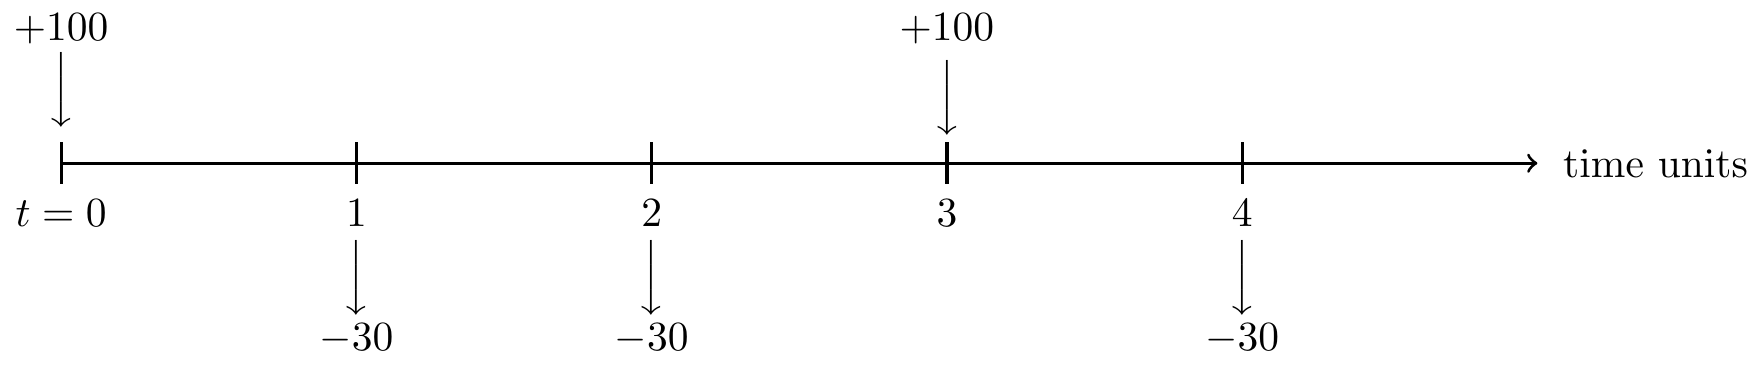
\includegraphics{SCMA329ExcelBookdownproj_files/figure-latex/tikz-exam1-1} \end{center}

\begin{enumerate}
\def\labelenumi{\arabic{enumi}.}
\setcounter{enumi}{2}
\item
  The effective rate of interest is 6\% per time unit. Cashflows are
  shown in the following time line.

  \begin{enumerate}
  \def\labelenumii{\arabic{enumii}.}
  \item
    Calculate the accumulation at time time t = 5 units of these
    cashflows.
  \item
    Calculate the value at time time t = 2 units of these cashflows.
  \item
    Calculate the present value at time time t = 0 units of these
    cashflows.
  \end{enumerate}
\end{enumerate}

\begin{center}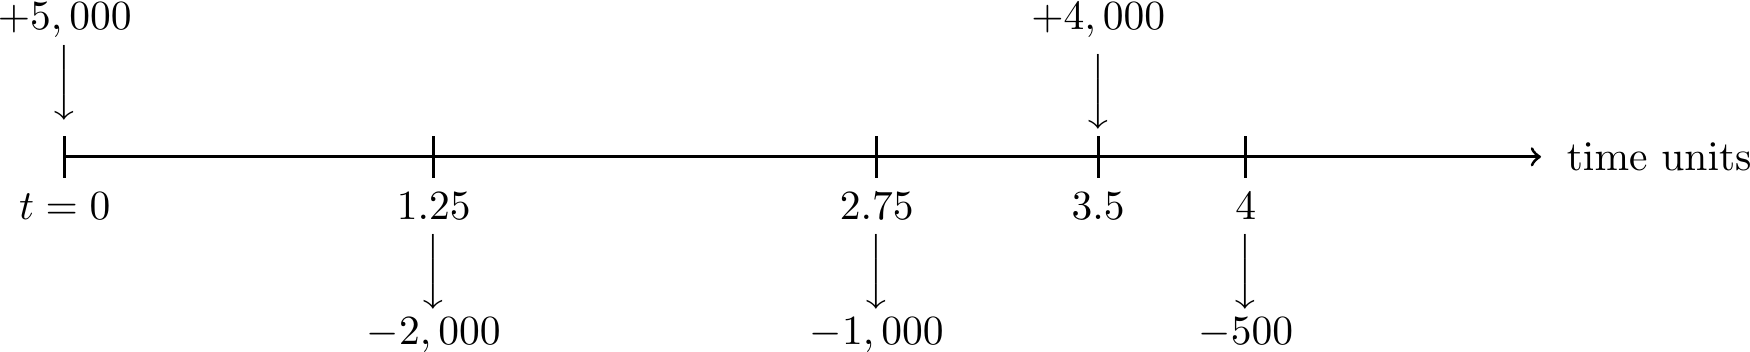
\includegraphics{SCMA329ExcelBookdownproj_files/figure-latex/tikz-exam2-1} \end{center}

\begin{enumerate}
\def\labelenumi{\arabic{enumi}.}
\setcounter{enumi}{3}
\item
  The effective rate of interest per annum was 4\% during 2015, 3\% per
  half-year until 1 October 2017 and 1.5\% per month thereafter.
  Cashflows are shown in the following time line.

  \begin{enumerate}
  \def\labelenumii{\arabic{enumii}.}
  \item
    Calculate the accumulation on 1/1/2019 of these cashflows.
  \item
    Calculate the present value on 1/1/2015 of these cashflows.
  \item
    Calculate the value at time time 1/7/2017 of these cashflows.
  \end{enumerate}
\end{enumerate}

\begin{center}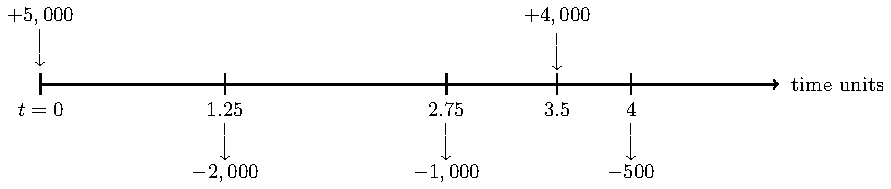
\includegraphics{SCMA329ExcelBookdownproj_files/figure-latex/tikz-exam3-1} \end{center}

\begin{enumerate}
\def\labelenumi{\arabic{enumi}.}
\setcounter{enumi}{4}
\tightlist
\item
  (Excel) It is a good exercise to check whether the Excel worksheet
  you have developed so far for calculating the present value and
  future value can be applied to the questions in this Tutorial. What
  would you do to improve the Excel worksheet for a more general
  scenario?
\end{enumerate}

\hypertarget{tutorial-3}{%
\section{Tutorial 3}\label{tutorial-3}}

\begin{enumerate}
\def\labelenumi{\arabic{enumi}.}
\item
  Calculate the present value now of an annuity payable monthly in
  advance. The annual amount of the annuity will be \$ 2,400 for the
  first 10 years and \$ 3,600 for the next 15 years, after which
  payment will cease. Assume that the effective rate of interest is 2\%
  per annum.
\item
  Assume that the effective rate of interest will be 3\% for 5 years
  from now, 4\% for the next 5 years and 5\% thereafter. Calculate the
  following values:

  \begin{enumerate}
  \def\labelenumii{\arabic{enumii}.}
  \item
    The present value of an annuity of \$ 1,000 per annum, payable
    in arrear for 15 years.
  \item
    The present value of an annuity due of \$ 500 per annum, payable
    at the beginning of the year for 20 years.
  \item
    The accumulation value of an increasing annuity payable yearly
    in arrear for 30 years. The first annual payment is \$ 100, and
    payments will be increase by \$ 100 each year.
  \item
    The accumulation value of an increasing annuity payable yearly
    in advance for 18 years. The first annual payment is \$ 1,000,
    and payments will be increase by 2\% each year (compound).
  \item
    The present value of an annuity of \$ 200, payable in arrear for
    10 years and deferred for 3 years.
  \end{enumerate}
\item
  You borrow \$ 240,000 from a bank to be repaid by the end of 5
  years. Assume that the interest rate is 4\% per annum. Consider the
  following four possible options for the loan to be repaid.

  \begin{enumerate}
  \def\labelenumii{\arabic{enumii}.}
  \item
    Calculate the amount of the repayments to repay if you choose to
    repay the loan as late as possible.
  \item
    You may choose to repay interest only during the 5 years term of
    loan and repay the capital at the end of the term. Calculate
    interest to be repaid and draw the timeline to illustrate the
    cashflows for the repayment of the loan.
  \item
    Calculate the amount X of level instalments to repay the loan
    which will be paid at the end of each year for 5 years and draw
    the timeline to illustrate the cashflows for the repayment of
    the loan.
  \item
    Calculate the amount Y of level instalments to repay the loan
    which will be paid at the end of each month for 5 years and draw
    the timeline to illustrate the cashflows for the repayment of
    the loan. \textbf{Instalment} is a sum of money due as one of several
    equal payments for something, spread over an agreed period of
    time.
  \end{enumerate}
\item
  A person now age 30 has received a pension from a company. When he
  retires at age 60, he will be paid on each birthday from the 60 to
  the 85th inclusive. The first annual payment will be half of his
  salary when he retires, and payments will then increase by 2\%
  compounding each year. Currently, he receive a salary of \$ 20,000
  and will increase by 3\% each year compounding in line with
  inflation. Assume that the effective rate of interest will be 4\% for
  the next 20 years and 5\% thereafter. Calculate the present value now
  of this pension.
\item
  (Excel) Use Excel worksheet you have developed so far to calculate
  the results from the questions in this Tutorial.
\end{enumerate}

\hypertarget{tutorial-4}{%
\section{Tutorial 4}\label{tutorial-4}}

\begin{enumerate}
\def\labelenumi{\arabic{enumi}.}
\item
  Show that the following series of cashflows are equivalent given
  that an interest rate is 4\% per annum effective.

  \begin{enumerate}
  \def\labelenumii{\arabic{enumii}.}
  \item
    One single payment of amount 14,802.44 at year 10.
  \item
    a level annuity of 400 payable yearly in arrear for the next 10
    years plus a lump sum of 10,000.
  \item
    a level annuity of 1,232.91 payable yearly in arrear for the
    next 10 years.
  \end{enumerate}
\item
  You invest in a project which requires you to pay 2,000 and receive
  back 300 at the end of each of the next 8 years. Calculate the yield
  of this investment. ANS = 4.2394551\%
\item
  You pay a price of 5,000 for an investment that will repay you 600
  per annum payable half-yearly in arrear for the next 12 years.
  Calculate the yield of this investment. ANS = 3.1491266\%
\item
  An investor pays 100,000 in order to receive 20,000 back at the end
  of the first 3 years and 25,000 back at the end in the next 4 years.
  Calculate the yield of this investment. ANS = 12.6209232\%
\item
  You invest in a project which requires you to pay 500,000 at the
  start of each of the calendar years 2018, 2019 and 2020. The project
  is expected to return profits of 400,000 for 6 years a the end of
  each calendar year 2024 to 2029 inclusive. Calculate the yield of
  this investment. ANS = 5.7285486\%
\item
  (Modified from CT1 2014 IFoA Exam)

  An investor is considering two projects, Project A and Project B.
  Project A involves the investment of 2,000,000 in a retail outlet.
  Rent is received quarterly in arrear for 25 years, at an initial
  rate of 100,000 per annum. It is assumed that the rent will increase
  at a rate of 5\% per annum compound, but with increases taking place
  every five years. Maintenance and other expenses are incurred
  quarterly in arrear, at a rate of 12,000 per annum. The retail
  outlet reverts to its original owner after 25 years for no payment.

  Project B involves the purchase of an office building for 1,000,000.
  The rent is to be received quarterly in advance at an initial rate
  of 85,000 per annum. It is assumed that the rent will increase to
  90,000 per annum after 20 years. There are no maintenance or other
  expenses. After 25 years the property reverts to its original owner
  for no payment.

  Calculate the annual effective internal reate of return for both
  Projects A and B. Which project is preferable?
\item
  (Excel) Use Excel worksheet you have developed to calculate the
  results from the questions in this Tutorial.
\end{enumerate}

\hypertarget{tutorial-5}{%
\section{Tutorial 5}\label{tutorial-5}}

\begin{enumerate}
\def\labelenumi{\arabic{enumi}.}
\item
  You borrow 30,000 for a term of 6 months to be repaid in arrear by
  level monthly instalments. The rate of interest will be 4\% pa
  effective.

  \begin{enumerate}
  \def\labelenumii{\arabic{enumii}.}
  \item
    Calculate the monthly repayment.
  \item
    Construct the complete loan schedule
  \end{enumerate}
\item
  A loan of 800,000 is repayable by equal monthly repayments for 10
  years, with interest rate payable at 6.5\% pa effective.

  \begin{enumerate}
  \def\labelenumii{\arabic{enumii}.}
  \item
    Calculate the amount of each monthly payment.
  \item
    Calculate the interest and capital contents of the 96th
    repayment.
  \end{enumerate}
\item
  \begin{enumerate}
  \def\labelenumii{\arabic{enumii}.}
  \item
    An investor takes out a loan of 100,000 from a bank to be repaid
    by level annual instalments in arrear over 12 years where the
    bank charges an effective annual rate of interest of 7\%.
    Immediately after the 6th repayment has been made, the investor
    may

    \begin{enumerate}
    \def\labelenumiii{\arabic{enumiii}.}
    \item
      extend the term of the loan by extra 2 year, or
    \item
      miss the next two repayments.
    \end{enumerate}

    Calculate the revised repayment amount in each case.
  \item
    Suppose the bank allows the
    investor to miss the next two repayments but the capital
    outstanding will be charged interest at 10\% pa effective while
    the investor is not making repayments. Calculate the revised
    repayment.
  \item
    Suppose in Question 3.2 that the investor will miss the next two
    repayment and extend the term of the loan by extra 4 years.
    Calculate the revised repayment.
  \end{enumerate}
\item
  An investor borrows 50,000 for a term of 12 years. The rate of
  interest will be 4\% pa effective for the first 6 years and 5\% pa
  effective thereafter. The loan will be repaid level annual
  repayments for the first 6 years, and then increasing to twice the
  origin level for the last 6 years. Calculate the annual repayment.
\item
  An investor borrows 40,000 for a term of 10 years. The rate of
  interest will be 6.5\% pa effective The loan will be repaid level
  annual repayments, increasing at 2\% per annum.

  \begin{enumerate}
  \def\labelenumii{\arabic{enumii}.}
  \item
    Calculate the first annual repayment.
  \item
    Calculate the capital outstanding after the 7th repayment is
    made.
  \item
    Calculate the interest content of the 8th repayment.
  \end{enumerate}
\item
  (Excel) Suppose you borrow \(L\) from a bank to be repaid by the end
  of \(n\) years at an interest rate of \(i\%\) per annum effective. If
  you agree to repay the loan and the interest in equal annual
  instalments throughout term of loan and the first payment is made at
  the end of the first year.

  Create a model to produce a loan amortisation (or loan schedule)
  table. Make the interest rate, loan life, initial loan, and other
  necessary variables input variables. The loan amortisation table
  should include the following columns:

  \begin{itemize}
  \item
    The year-beginning balance
  \item
    The annual repayment
  \item
    Interest Component
  \item
    Capital content
  \item
    Capital outstanding (the year-end balance)
  \end{itemize}
\end{enumerate}

\hypertarget{solutions-to-tutorial-1}{%
\section{Solutions to Tutorial 1}\label{solutions-to-tutorial-1}}

\begin{enumerate}
\def\labelenumi{\arabic{enumi}.}
\item
  The solutions to each question are as follows:

  \begin{enumerate}
  \def\labelenumii{\arabic{enumii}.}
  \tightlist
  \item
    \(5000 (1.075)^4 = 6677.345703\)
  \item
    Let \(i\%\) be the annual rate effective equivalent to \(3\%\) per quarter-effective, \(i = (1.03)^4 - 1\).
    Hence, the accumulation is
    \[800(1+i)^{2.7} = 800(1.03)^{4\times2.7} = 1100.859802.\]
  \item
    Let \(j\%\) be the monthly rate effective equivalent to \(4.25\%\) per half-year effective, \(j = (1.0425)^{2/12} - 1\).
    Hence, the accumulation is
    \[10000(1.0425)^{(2/12)\times27} = 12059.86056.\]
  \end{enumerate}
\item
  The solutions to each question are as follows:

  \begin{enumerate}
  \def\labelenumii{\arabic{enumii}.}
  \tightlist
  \item
    \(\frac{1000}{1.075} = 930.232558\).
  \item
    \(\frac{100}{(1.03)^7} = 81.309151\).
  \item
    Let \(j\%\) be the quarterly rate effective equivalent to \(4.25\%\) per half-year effective, \(j = (1.0425)^{2/4} - 1\).
    Hence, the present value is
    \[10000\times (1+j)^{-5} = 10000(1.0425)^{-(5/2)} = 9011.764643.\]
  \end{enumerate}
\item
  The solutions to each question are as follows:

  \begin{enumerate}
  \def\labelenumii{\arabic{enumii}.}
  \tightlist
  \item
    0.3274\%
  \item
    3.1988\%
  \end{enumerate}
\item
  The solutions to each question are as follows:

  \begin{enumerate}
  \def\labelenumii{\arabic{enumii}.}
  \tightlist
  \item
    500(1.04)(1.05)(1.06) =578.76
  \item
    \(2000(1.04)^{3/4}(1.05)(1.06)^{3/4} =2259.299\)
  \item
    (1.04)(1.05)(1.06) = 1.15752
  \end{enumerate}
\item
  The account balance in 3 years is \(3000(1.025)^{3} = 3230.67\).
\item
  The amount to be repaid for the loan is 5000(1.1) = 5500.
\item
  Let \(X\) be the amount to be deposited now.
  \[X = \frac{1000}{(1.0575)^4} + \frac{2000}{(1.0575)^8} = 2078.36. \]
\item
  At time 3.75 years, Katy has a balance of \(100(1+i)^{15}\). The interest on this balance over the next 3 months is \(100(1+i)^{15}\cdot i\).
  Taylor earns simple interest on the original amount which is equal to \(500i\cdot\frac{3}{12}\). Therefore, we solve for \(i\) from the following equation:
  \[ 100(1+i)^{15}\cdot i = 500i\cdot\frac{3}{12},\] which gives \(i = 0.014987.\)
\item
  The timeline for the following annuity having cashflow of 1 unit at the end of each of the next \(n\) time units is given in the figure below:
\end{enumerate}

\begin{center}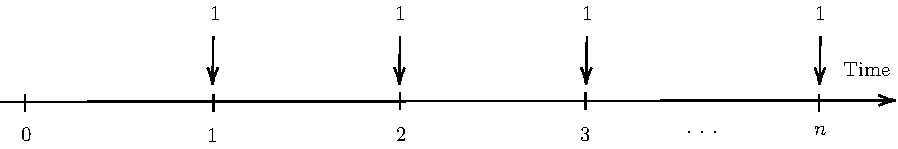
\includegraphics{SCMA329ExcelBookdownproj_files/figure-latex/tikz-sol1-1} \end{center}

\begin{enumerate}
\def\labelenumi{\arabic{enumi}.}
\setcounter{enumi}{9}
\tightlist
\item
  (More details in the course ``Life Contingencies I''). We need to define a random variable \(T_x\) = the remaining future life time of a life aged \(x\).
\end{enumerate}

\begin{center}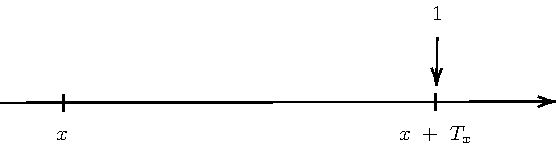
\includegraphics{SCMA329ExcelBookdownproj_files/figure-latex/tikz-sol2-1} \end{center}

The quantity of interest is the present value of the death benefit assuming the interest rate of \(i\%\) p.a. effective. It is also a random variable,
\[PV = \frac{1}{(1+i)^{T_x}}.\] It turns out that the premium rate of this whole life insurance is \(E[PV]\), the expected value of the present value, \(PV\).

\hypertarget{solutions-to-tutorial-2}{%
\section{Solutions to Tutorial 2}\label{solutions-to-tutorial-2}}

\begin{enumerate}
\def\labelenumi{\arabic{enumi}.}
\item
  The solutions to each question are as follows:

  \begin{enumerate}
  \def\labelenumii{\arabic{enumii}.}
  \tightlist
  \item
    \((1.03)^3(1.04)^{2.5} (1.02)^{12} = 1.528611\)
  \item
    \(5000A(0.5,2.75) = 5000(1.03)(1.04)^{2.5} (1.02)^{9} = 6788.786068\)
  \item
    We first find the rate \(j\%\) per month effective that is equivalent to the rate of \(4\%\) per half-year effective.
    \[j = (1.04)^{1/6} - 1 = 0.00656.\]
    The accumulated value is \(100A(1+2/12, 3 + 7/12 ) = 100(1+j)^{10}(1.02)^{19} = 155.522118.\)
  \item
    \(25000V(0,1.5) = \frac{25000}{(1.03)^3(1.04)^{1.5}} = 21571.39968.\)
  \item
    \(8000V(0.25,2.75) = \frac{8000}{(1.03)^2(1.04)^{2.5}(1.02)^{9}} = 5720.455921.\)
  \item
    \(V(0.5,1.75) = \frac{1}{(1.03)(1.04)^{2}} = 0.897627.\)
  \end{enumerate}
\item
  The solutions to each question are as follows:

  \begin{enumerate}
  \def\labelenumii{\arabic{enumii}.}
  \tightlist
  \item
    With \(i = 7.25\%\) per time period, \(V(4) = 100 (1+i)^4 - 30(1+i)^3 - 30 (1+i)^2 + 100 (1+i) - 30 = 138.041762.\)
  \item
    \(V(8) = V(4)\cdot (1+i)^4 = 182.641597.\)
  \item
    \(PV(0) = V(4)\cdot (1+i)^{-4} = 104.332903.\)
  \end{enumerate}
\item
  The solutions to each question are as follows:

  \begin{enumerate}
  \def\labelenumii{\arabic{enumii}.}
  \tightlist
  \item
    With \$ = 6\%\$ per time period, \(V(5) = 5000 (1+i)^5 - 2000(1+i)^{3.75} - 1000 (1+i)^{2.25} + 4000 (1+i)^{1.5} - 500(1+i) = 6897.948585.\)
  \item
    \(V(2) = V(5)(1+i)^{-3} = 5791.650645.\)
  \item
    \(PV(0) = V(5)(1+i)^{-5} = 5154.548456.\)
  \end{enumerate}
\item
  The solutions to each question are as follows:

  \begin{enumerate}
  \def\labelenumii{\arabic{enumii}.}
  \tightlist
  \item
    \(V(1/1/2019) = 100(1.04)(1.03)^{3.5}(1.015)^{15} - 30 (1.03)^{3.5} (1.015)^{15}- 30 (1.03)^{1.5} (1.015)^{15} + 100 (1.015)^{12} - 30 = 152.955693.\)
  \item
    \(PV(0)= V(1/1/2015) = \frac{152.955693}{(1.04)(1.03)^{3.5}(1.015)^{15}} =106.074596.\)
  \item
    \(V(1/7/2017) = PV(0)(1.04)(1.03)^3 = 120.546998.\)
  \end{enumerate}
\end{enumerate}

\hypertarget{solutions-to-tutorial-3}{%
\section{Solutions to Tutorial 3}\label{solutions-to-tutorial-3}}

\begin{enumerate}
\def\labelenumi{\arabic{enumi}.}
\tightlist
\item
  Let \(j\) be the effective rate per month equivalent to \(i = 2\)\%. We have
  \[ j = (1.02)^{1/12}  - 1= 0.001652. \]
  Hence,
\end{enumerate}

\[ PV(0) = 200 \ddot{a}^{j}_{120} + 300 \ddot{a}^{j}_{180} \left( \frac{1}{1.02} \right)^{10} = 60148.03. \]

\begin{enumerate}
\def\labelenumi{\arabic{enumi}.}
\setcounter{enumi}{1}
\item
  The solutions to each question are as follows:

  \begin{enumerate}
  \def\labelenumii{\arabic{enumii}.}
  \item
    The cashflows have been splitted into three periods: (a) from time point 0-5, (b) 5-10 and (c) time point 10 onward.
    \[PV(0) = 1000 ( a^{3\%}_{5} + 1.03^{-5} a^{4\%}_{5} +  1.03^{-5} 1.04^{-5} a^{5\%}_{5}) = 11489.49  \]
  \item
    We have
    \[PV(0) = 500 ( \ddot{a}^{3\%}_{5} + 1.03^{-5} \ddot{a}^{4\%}_{5} +  1.03^{-5} 1.04^{-5} \ddot{a}^{5\%}_{10}) = 7229.67  \]
  \item
    The accumuated value is
    \[100 (Is)^{3\%}_{5} (1.04)^5 (1.05)^{20} + \left[100 (Is)^{4\%}_{5} + 500 s^{4\%}_{5} \right] (1.05)^{20}  + \left[100 (Is)^{5\%}_{20} + 1000 s^{5\%}_{20} \right]= 78929.01  \]
  \item
    Let \(i_1 = 3\%, i_2 = 4\%\) and \(i_3 = 5\%\). The accumuated value is given by
    \[\begin{aligned} 
     V(18) &= \left[1000(1+i_1)^5 + 1000(1.02)(1+i_1)^4 + 1000(1.02)^2(1+i_1)^3 + \ldots + 1000(1.02)^4(1+i_1)\right](1.04)^5(1.05)^8   \\
     &+ \left[1000(1.02)^5(1+i_2)^5 + 1000(1.02)^6(1+i_2)^4 + 1000(1.02)^7(1+i_2)^3 + \ldots + 1000(1.02)^9(1+i_2)\right](1.05)^8   \\
     &+ \left[1000(1.02)^{10}(1+i_3)^8 + 1000(1.02)^{11}(1+i_3)^7 + 1000(1.02)^{12}(1+i_3)^6 + \ldots + 1000(1.02)^{17}(1+i_3)\right]  \\
     &= 1000(1.02)^5 \left[ \left(\frac{1+i_1}{1.02}\right)^5   + \left(\frac{1+i_1}{1.02}\right)^4 + \ldots + \left(\frac{1+i_1}{1.02}\right) \right](1.04)^5(1.05)^8 \\
     &+ 1000(1.02)^{10} \left[ \left(\frac{1+i_2}{1.02}\right)^5   + \left(\frac{1+i_2}{1.02}\right)^4 + \ldots + \left(\frac{1+i_2}{1.02}\right) \right](1.05)^8 \\
      &+ 1000(1.02)^{18} \left[ \left(\frac{1+i_3}{1.02}\right)^8   + \left(\frac{1+i_3}{1.02}\right)^7 + \ldots + \left(\frac{1+i_3}{1.02}\right) \right] 
     \end{aligned}\]
    Let \(1+j_1 = \frac{1+i_1}{1.02}\). Then, \(j_1 = 0.009804\) and
    \[ \left[ \left(\frac{1+i_1}{1.02}\right)^5   + \left(\frac{1+i_1}{1.02}\right)^4 + \ldots + \left(\frac{1+i_1}{1.02}\right) \right] = \frac{(1+j_1)^5 - 1}{j_1/(1+j_1)} = 5.148995.\]
    Let \(1+j_2 = \frac{1+i_2}{1.02}\). Then, \(j_2 = 0.019608\) and
    \[ \left[ \left(\frac{1+i_2}{1.02}\right)^5   + \left(\frac{1+i_2}{1.02}\right)^4 + \ldots + \left(\frac{1+i_2}{1.02}\right) \right] = 5.301921.\]
    Let \(1+j_3 = \frac{1+i_3}{1.02}\). Then, \(j_3 = 0.029412\) and
    \[ \left[ \left(\frac{1+i_3}{1.02}\right)^8   + \left(\frac{1+i_3}{1.02}\right)^7 + \ldots + \left(\frac{1+i_3}{1.02}\right) \right]  = 9.134790.\]
    Therefore, \(V(18) = 32814.45\).
  \item
    The present value is
  \end{enumerate}
\end{enumerate}

\[\begin{aligned}
    PV(0) &= \left( \frac{200}{(1.03)^4} + \frac{200}{(1.03)^5}\right) + 200 a^{0.04}_5 (1.03)^{-5} + 200 a^{0.05}_{3} (1.03)^{-5} (1.04)^{-5} \\
    &= 350.2192 + 768.0362 + 386.1574 = 1504.413
\end{aligned}\]

\begin{enumerate}
\def\labelenumi{\arabic{enumi}.}
\setcounter{enumi}{2}
\item
  The solutions to each question are as follows:

  \begin{enumerate}
  \def\labelenumii{\arabic{enumii}.}
  \tightlist
  \item
    \(240000 (1.04)^5 = 291996.7\)
  \item
    The interest amounts are \(0.04\times 240000 = 9600.\)
  \item
    By the Principle of Equivalence, we have
    \[ 240000 = X a^{0.04}_{5}. \]
    This gives X = 53910.51.
  \item
    Level installments are payable monthly, which follows
    \[ 240000 = Y a^{j}_{60}, \]
    where \(j = (1.04)^{1/12} - 1\). This gives Y = 4412.23.
  \end{enumerate}
\item
  The person retires in 30 years, when his salary is expected to be
  \(20000 \times (1.03)^{30} = 48545.25.\)
  The first payment will be half of this which is equal to 24272.62.
  The present value at age 60 of his pension is
  \[  24272.62 \times \ddot{a}^{0.029412}_{26} = 449717.9\] (the precise value is 449719.051954).
  Here we use \(\frac{1.05}{1.02} = 1.029412\) and the annuity is paid from the 60th to the 85th birthday inclusive so there are 26 payments made in advance.
  Therefore, the present value of this at age 30 is
  \[ 449717.9 \times (1.05)^{-10} \times (1.04)^{-20} = 126002.9. \]
  (the precise value is 126003.181173)
\end{enumerate}

\hypertarget{solutions-to-tutorial-4}{%
\section{Solutions to Tutorial 4}\label{solutions-to-tutorial-4}}

\begin{enumerate}
\def\labelenumi{\arabic{enumi}.}
\item
  To examine whether the cashflows are equivalent, we compare their present values.

  \begin{enumerate}
  \def\labelenumii{\alph{enumii}.}
  \item
    The present value of single payment of amount 14,802.44 at year 10 is
    \[ PV(0) =  \frac{14,802.44}{1.04^{10}} = 10000.\]
  \item
    The present value of the level annuity of 400 payable yearly in arrears for the next 10 years plus a lump sum of 10,000 is
    \[ PV(0) =  400 a^{0.04}_{10} +\frac{10000}{1.04^{10}} = 10000.\]
  \item
    The present value of the level annuity of 1,232.91 payable yearly in arrears for the next 10 years.
    \[ PV(0) =  1,232.91 a^{0.04}_{10}  = 10000.\]
  \end{enumerate}
\end{enumerate}

It follows that the values of these cashflows are the same, i.e.~equivalent.

\begin{enumerate}
\def\labelenumi{\arabic{enumi}.}
\setcounter{enumi}{1}
\item
  The annual yield of this investment \(i\) is the solution of the equation of value:
  \[ f(i) = -2000(1+i)^8 +300 s^i_8 = 0. \]
  If we solve using software, we get \(i = 4.2394551%
  \). Instead of using software, you can also use linear interpolation to approximate the solution.
\item
  Working in time unit of half year, the equation of value is
  \[ f(i) = -5000(1+i)^{12 \times 2} + 300 s^i_{24} = 0. \]
  The yield \(i\) per half year is \(i = 3.1491266\%\) and hence the annual yield is \(6.397423\%.\)
\item
  The equation of value is
  \[ f(i) = -100(1+i)^{7} + 20 s^i_{7}  + 25 s^i_{4} = 0. \]
  The annual yield is \(12.6209232\%.\)
\item
  You are suggested to draw the time line for these cashflows. The equation of value is
  \[ f(i) = -5 \ddot{s}^i_{3}(1+i)^{9}   + 4 s^i_{6} = 0. \]
  The annual yield is \(5.7285486\%.\)
\end{enumerate}

\hypertarget{solutions-to-tutorial-5}{%
\section{Solutions to Tutorial 5}\label{solutions-to-tutorial-5}}

\begin{enumerate}
\def\labelenumi{\arabic{enumi}.}
\tightlist
\item
  The monthly repayment can be calculated from this equation
  \[ X = \frac{30000}{a^j_6} = \frac{30000}{5.931847} = 5057.45,\]
  where \(j = (1.04)^{1/12} - 1 = 0.003274.\)
\end{enumerate}

The complete loan schedule is illustrated below:

\begin{longtable}[]{@{}ccccc@{}}
\toprule
Time & Repayment & Interest Content & Capital Content & Capital Outstanding \\
\midrule
\endhead
0 & - & - & - & 30000 \\
1 & \(X\) & 98.21 & 4959.23 & 25040.77 \\
2 & \(X\) & 81.98 & 4975.47 & 20065.30 \\
3 & \(X\) & 65.69 & 4991.76 & 15073.54 \\
4 & \(X\) & 49.35 & 5008.10 & 10065.44 \\
5 & \(X\) & 32.95 & 5024.50 & 5040.94 \\
6 & \(X\) & 16.50 & 5040.94 & 0 \\
\bottomrule
\end{longtable}

\begin{enumerate}
\def\labelenumi{\arabic{enumi}.}
\setcounter{enumi}{1}
\tightlist
\item
  The monthly repayment can be calculated from this equation
  \[ X = \frac{800000}{a^j_{120}} = \frac{800000}{88.806749} = 9008.32,\]
  where \(j = (1.065)^{1/12} - 1 = 0.005262.\)
\end{enumerate}

The capital outstanding after 95th repayment (25 payments left) is
\[ L_{95} = 9008.32 a^j_{25} = 210506.84.  \]

Hence, the interest content of the 96th repayment is
\[ j \times L_{95} = 0.005262 \times 210506.84 = 1107.62.\]
The capital content of the 96th repayment is
\[ X - 1107.62 = 7900.70. \]

\begin{enumerate}
\def\labelenumi{\arabic{enumi}.}
\setcounter{enumi}{2}
\item
  \begin{enumerate}
  \def\labelenumii{\arabic{enumii}.}
  \tightlist
  \item
  \end{enumerate}

  \begin{enumerate}
  \def\labelenumii{\alph{enumii}.}
  \item
    \textbf{Extending the term of the loan by extra 2 year:} The original repayment is
    \[ X = \frac{100000}{a^{0.07}_{12}} = \frac{100000}{7.942686} = 12590.20,\]
    The capital outstanding after 6th repayment (6 payments left) is
    \[ L_{6} = X a^{0.07}_{6} = 60011.68.  \]
    By extending the term of the loan by extra 2 year, the revised repayment \(X'\) can be obtained (for 8 payments) from
    \[ X' = \frac{L_6}{a^{0.07}_{8}} = 10050.02\]
  \item
    \textbf{Missing the next two repayments:} From the previous result, the capital outstanding after 6th repayment \(L_6 = 60011.68\). Then in 2 years, with interest at \(7\%\) per annum, this accumulates to
    \[ L_6 \times (1.07)^2 = 68707.37. \]
    This must now be repaind by only 4 annual repayments, so the new repayment \(X''\) can be obtained from
    \[ X'' = \frac{68707.37}{a^{0.07}_{4}} = 20284.35.\]
  \end{enumerate}

  \begin{enumerate}
  \def\labelenumii{\arabic{enumii}.}
  \setcounter{enumii}{1}
  \tightlist
  \item
    The capital outstanding will accumulate (at \(10\%\)) to
    \[ L_6 \times (1.1)^2 = 72614.14. \]
  \end{enumerate}

  The new repayment amount \(X'''\) is
  \[X''' = \frac{72614.14}{a^{0.07}_{4}} = 21437.73.\]

  \begin{enumerate}
  \def\labelenumii{\arabic{enumii}.}
  \setcounter{enumii}{2}
  \tightlist
  \item
    The new repayment amount will be
    \[\frac{72614.14}{a^{0.07}_{8}} = 12160.53.\]
  \end{enumerate}
\item
  You are suggested to draw the time line for these cashflows. Let \(X\) be the level of repayment of the first 6 years (\(2X\) will be repaid after this period for the last 6 years). It can be obtained from
  \[ 50000 = X(a^{0.04}_6 + 2 a^{0.05}_6 (1.04)^{-6}) = 3769.34.\]
\item
  \begin{enumerate}
  \def\labelenumii{\arabic{enumii}.}
  \tightlist
  \item
    Let \(X\) be the first annual repayment. Then,\\
    \[ 40000 = X(v + v^2(1.02) + v^3(1.02)^2 + \ldots + v^{10}(1.02)^9),\]
    where \(v = 1/(1.065).\) By rewriting the above equation, we have
    \[ 40000 = \frac{X}{1.02}(\frac{1.02}{1.065} + \left( \frac{1.02}{1.065} \right)^2 + \left( \frac{1.02}{1.065} \right)^3 + \ldots + \left( \frac{1.02}{1.065} \right)^{10}),\]
  \end{enumerate}

  Let \(i' = \left( \frac{1.065}{1.02} -1 \right) = 0.044118.\) Hence,
  \[ 40000 = \frac{X}{1.02} \cdot a^{i'}_{10},\]
  and \(X = 5133.91.\)

  \begin{enumerate}
  \def\labelenumii{\arabic{enumii}.}
  \setcounter{enumii}{1}
  \tightlist
  \item
    We will calculate the capital outstanding after 7th repayment, \(L_7\) (3 payments left). We first find the amount \(X_8\)of the 8th repayment,
    \[X_8 = X(1.02)^7 = 5897.25.\]
  \end{enumerate}

  So the capital outstanding after the 7th repayment is equal to the present value of the remaining 3 repayments (see the table below).
\end{enumerate}

\begin{longtable}[]{@{}ccccc@{}}
\toprule
Time & 7 & 8 & 9 & 10 \\
\midrule
\endhead
Payment & \(L_7 = ?\) & \(X_8\) & \(X_8 (1.02)\) & \(X_8(1.02)^2\) \\
\bottomrule
\end{longtable}

It follows that
\[
\begin{aligned} L_7 &= X_8( v + v^2 + v^3) \\
&= \frac{X_8}{(1.02)} a^{i'}_3 \\
&= 15919.94,
\end{aligned}\]
where \(v\) and \(i'\) are the same as above.

\begin{enumerate}
\def\labelenumi{\arabic{enumi}.}
\setcounter{enumi}{2}
\tightlist
\item
  The interest content of the 8th repayment is
  \[ L_7 * i = 15919.94 \times 0.065 = 1034.80.\]
\end{enumerate}

\end{document}
